\section[Background]{Background\footnote{Content taken from~\cite{manual}, if not noted otherwise.}}
\subsection{Cosmic Expansion}
A spatially homogeneous and isotropic Universe can be described as FLRW metric. Solving Einstein's field equations with FLRW metric gives expansion of the Universe~\cite{TEU}. Hubble parameter $H(t)=\dot{a}(t)/a(t)$ evolves according to
\begin{equation}
   H^2(t) = H_0^2 \left[ \Omega_\text{rad} a^{-4}(t) + \Omega_\text{mat}a^{-3}(t) + \Omega_\text{curv}a^{-2} (t) + \Omega_\Lambda \right]
\end{equation}

Because of expansion of the Universe, light emitted in the past gets redshifted over time. The redshift of a source is given by,
\begin{equation}
   z=\frac{\lambda_\text{obj}-\lambda_\text{em}}{\lambda_\text{em}}
\label{math:z}
\end{equation}
\noindent
Where, $\lambda_\text{obs}$ and $\lambda_\text{em}$ are, respectively, the wavelengths at time of observation and emission.
Redshift is directly related to the scale factor by,
\begin{equation}
1+z=\frac{1}{a(t_{em})}
\end{equation}
with scale factor at present time defined as $a(t_0) = 1$.

The local Hubble law are given by the following formula,\\
 \begin{equation}
    v_\text{esc}=H_{0}D
 \label{Hubble}
 \end{equation}
 where, $H_{0} = H(t_0)$ is Hubble constant and $D$ is the distance between object and observer.
  
  \subsection{Distances}
  Accordingly, one defines the angular diameter distance as exactly this ratio,
  \begin{equation}
  	D_\text{ang}(z)=2R/\delta=a(z)f_{K}(w)
  \label{DAngular}
  \end{equation}
  \noindent
  Where, $R$ is the radius of the distant object, $\delta$ is the angular diameter, and $z$ is the cosmological redshift. If we consider an observer at redshift $ z_{1} $ gives the angular diameter of another object at redshift $ z_{2} $, so equation \ref{DAngular} becomes
  \begin{equation}
  D_\text{ang}(z_{1},z_{2})=a(z_{2})f_{K}[w(z_{2}) - w(z_{1})]
  \label{math:Dangular2}
  \end{equation}
  Another distance measure relates the observed flux, S, of a source to its luminosity, L. For a known luminosity, the distance to the source can be determined as,
  \begin{equation}
  D_\text{lum}(z)=\sqrt{\frac{L}{4\pi S}}
  \end{equation}
  
  \subsection{Quasars}
  
  \subsection{Gravitational lensing}
  
  \begin{figure}[ht]
  	\centering
     % 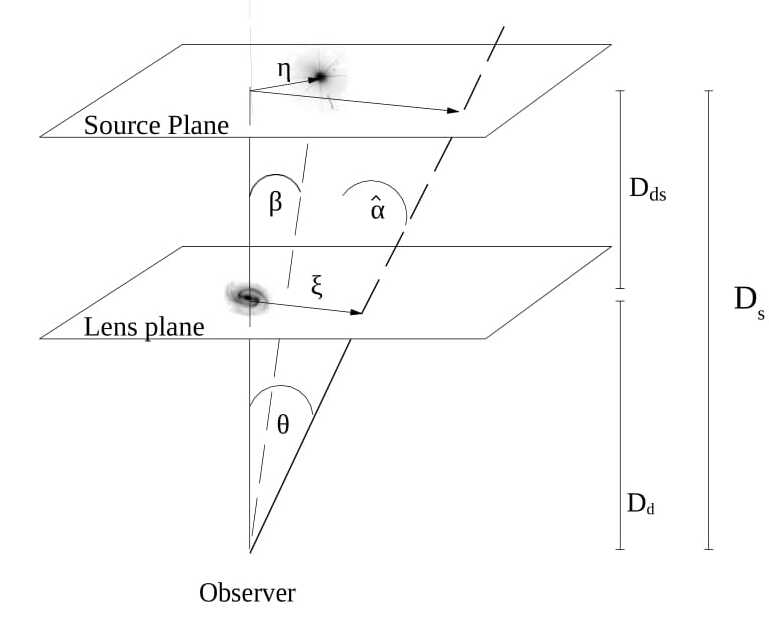
\includegraphics[width=0.5\linewidth]{./figs/lensing.png}
   \caption{Schematic diagram of the gravitational lensing system~\cite{wiki}. \textcolor{blue}{picture and citation missing!}}%
  	\label{fig:lensing}
  \end{figure}
  
\subsubsection{Lens Equation}
For simplicity, we assume that all angles considers are small so that $\tan x \approx \sin x \approx x$, source plane and lens plane are parallel, and light travles in straight line in between planes.For a given source, the lens equation is given by,
\begin{equation}
\pmb\beta = \pmb\theta - \pmb\alpha (\pmb\theta)
\label{LEquation}
\end{equation}
\noindent
where, $\pmb\theta$ is the apparent angular position of the source in the sky, $\pmb\beta$ is its true position, and $\pmb\alpha $ is the scaled deflection angle.

Now, we can define a dimensionless surface mas density with convergence as,
\begin{equation}
\kappa(\pmb\theta)=\frac{\sum(D_{d} \pmb \theta)}{\sum_\text{cr}}
\label{Equ:KTheta}
\end{equation}
with the critical surface mass density,
 \begin{equation}
 \Sigma_\text{cr}=\frac{c^2}{4\pi G}\frac{D_{s}}{D_{d}D_{ds}}
 \label{SumCr}
 \end{equation}
 
The scaled deflection angle can be rewritten as,
\begin{equation}
   \pmb\alpha(\pmb\theta)=\frac{1}{\pi}\int \dd[2]{\theta'} \kappa(\pmb{\theta}')\frac{\pmb\theta-\pmb\theta'}{| \pmb\theta -\pmb\theta'| ^2}
\label{ScaledDA}
\end{equation} 
For further convenience, a deflection potential is introduced
\begin{equation}
   \psi(\pmb\theta)=\frac{1}{\pi}\int \dd[2]{\theta'} \kappa(\pmb\theta') \ln | \pmb\theta- \pmb\theta'| 
\label{psiTheta}
\end{equation}

The use of this quantity is well-motivated because it encloses all information of the mass distribution of the lens~\cite{manual}. In addition, relation of deflection potential and deflection angle can be found
\begin{equation}
\pmb\alpha(\pmb\theta)=\pmb\nabla\psi(\pmb\theta)
\label{Equ:AlphaTheta}
\end{equation}
From the deflection potential a further scalar function, the Fermat potential, can be defined
\begin{equation}
\tau(\pmb\theta; \pmb\beta)=\frac{1}{2}(\pmb\beta -\pmb\theta)^2 -\psi(\pmb\theta)
\label{Equ:Format}
\end{equation}

Finally to find the magnification of the images is given by
\begin{equation}
\mu =(det A)^{-1}
\end{equation}
where, \text{A} is the Jacobian matrix of lens mapping.
\begin{equation}
A_{ij}=\frac{\partial\beta_{i}}{\partial \theta_{j}}
\end{equation}

\subsubsection{The SIS (Singular Isothermal Sphere)}
A simple model to describe the mass distribution of a galaxy acting as a lens is the singular isothermal sphere (SIS):
\begin{equation}
\rho(r)=\frac{\sigma_{v}^{2}}{2\pi G r^2}
\label{equ:SIS}
\end{equation}
where $ \sigma_{v} $ is the velocity dispersion. Physically this means that the lens system consists of self-gravitating with Maxwellian velocity distribution~\cite{Schneider}.

Integration along the line of sight yields the surface mass density
\begin{equation}
\Sigma(\xi)=\frac{\sigma^2_{v}}{2G\xi}
\label{equ:Sigma(xi)}
\end{equation}

\noindent
A characteristic angular scale of an axisymmetric lens is given by the Einstein radius $ \theta_{E} $ , defined as the angle inside which the mean of the convergence is unity. As a consequence, the projected mass inside $ \theta_{E} $ can be written as,
\begin{equation}
M(\theta \le \theta_{E})=\pi \theta^2_{E}D^2_{d}\Sigma_{cr}
\end{equation}

For an SIS the Einstein radius reads
\begin{equation}
\theta_{E}=4\pi\bigg( \frac{\sigma_{v}}{c}\bigg)^2\frac{D_{ds}}{D_{s}}
\label{Equ:ThetaE}
\end{equation}

\subsection{Calibration frames}
\subsection{Image reduction}
